\documentclass{fkssolpub}

\usepackage[czech]{babel}
\usepackage{fontspec}
\usepackage{fkssugar}
\usepackage{amsmath}
\usepackage{graphicx}

\author{Ondřej Sedláček}
\school{Gymnázium Oty Pavla} 
\series{3p}
\problem{6} 

\begin{document}

\begin{figure}[h!]
	\centering
	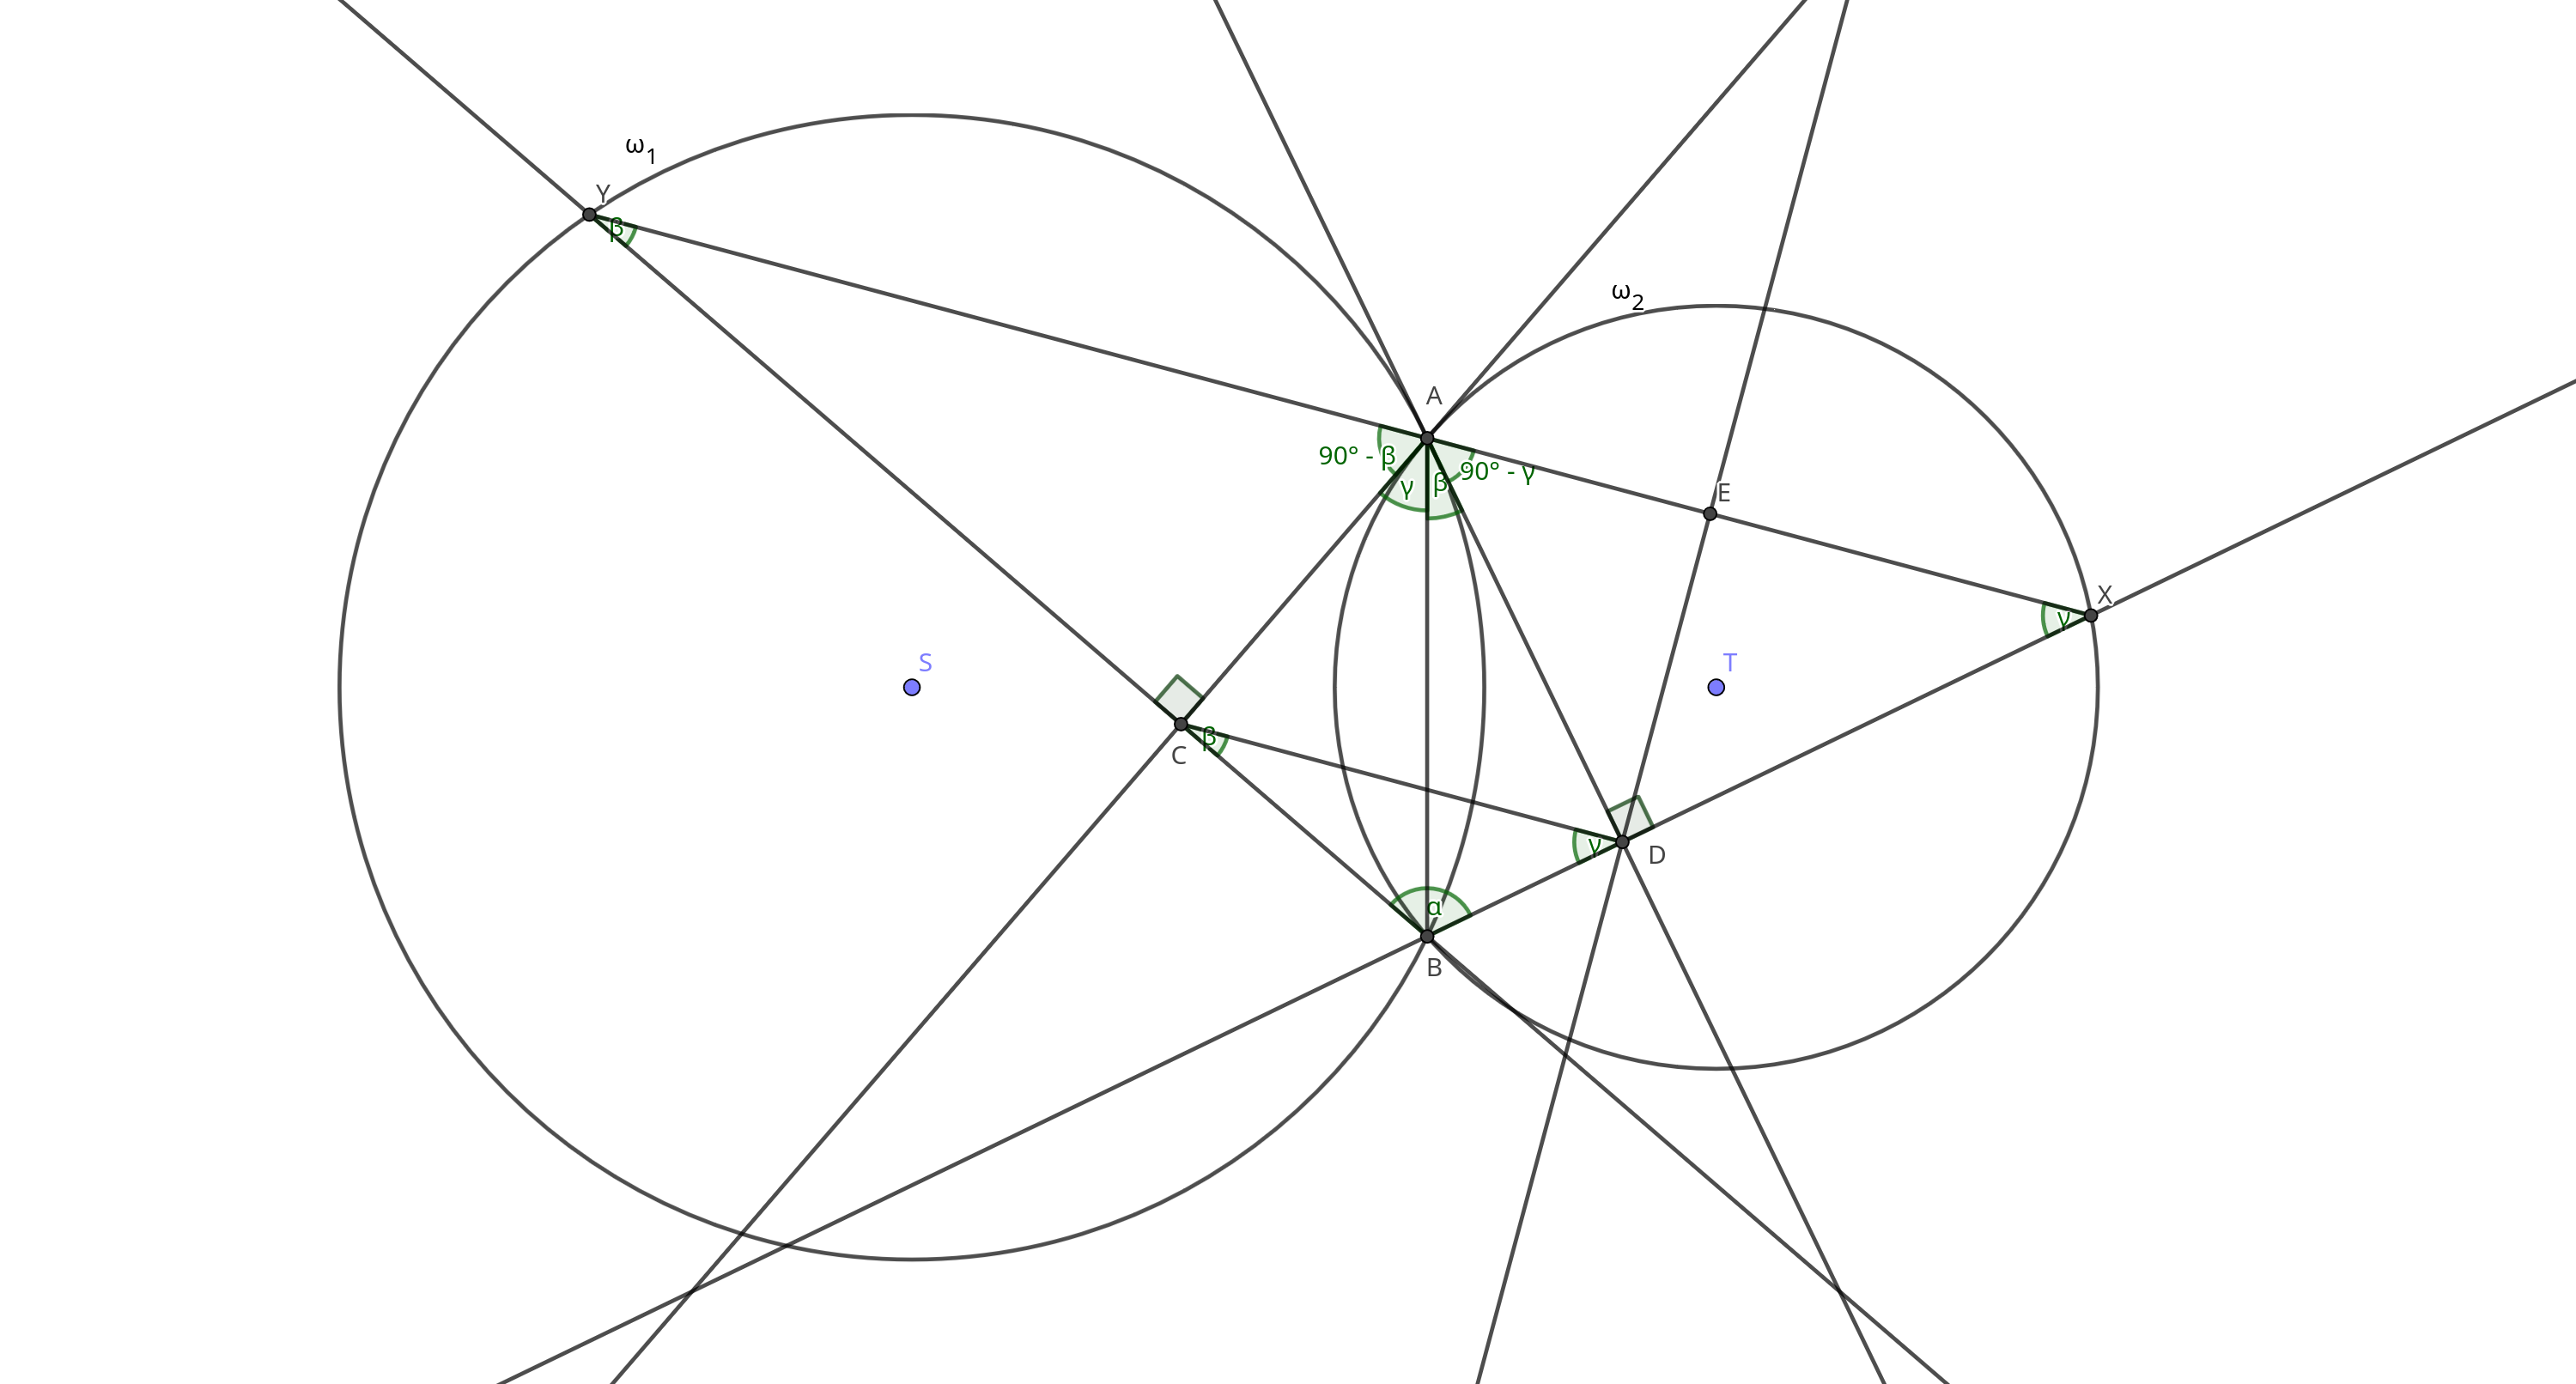
\includegraphics[width=\textwidth]{6-fig.png}
	\caption{Konstrukce zadání s dopočítanými úhly}
\end{figure}

Nechť $|\angle l_2; AB| = \gamma$ a $|\angle AB; l_1| = \beta$. Můžeme si
pak všimnout, že pro trojúhelník $BAY$ je velikost úsekového úhlu $\beta$
a pro trojúhelník $ABX$ je velikost úsekového úhlu $\gamma$, díky čemuž
$|\angle AYB| = \beta$ a $|\angle BXA| = \gamma$. Ze zadání pak víme,
že $l_1 \perp BX$ a $l_2 \perp BY$, a když označíme postupně průsečíky
kolmic jako $D$, $C$, dopočítáme $|\angle XAD| = 90^{\circ} - \gamma$
a $|\angle CAY| = 90^{\circ} - \beta$. Teď už můžeme získat $|\angle YAX|
	= 180^{\circ}$, z čehož vyplývá, že body $X$, $Y$ a $A$ leží na jedné
přímce. Q. E. D.

\end{document}
